\section{第三章：實驗 2 結果與厚度鎖死評估}
\label{sec:thickness_locking}

\subsection{數值結果與圖表展示}
在固定 $17 \times 17$ 網格條件下，跨越 5 個數量級的板厚度掃描實驗所得出的位移場與轉角場全域高斯相對 $L_2$ 誤差波動圖如圖 \ref{fig:thickness_error} 所示。

\begin{figure}[H]
    \centering
    \begin{subfigure}[b]{0.48\textwidth}
        \centering
        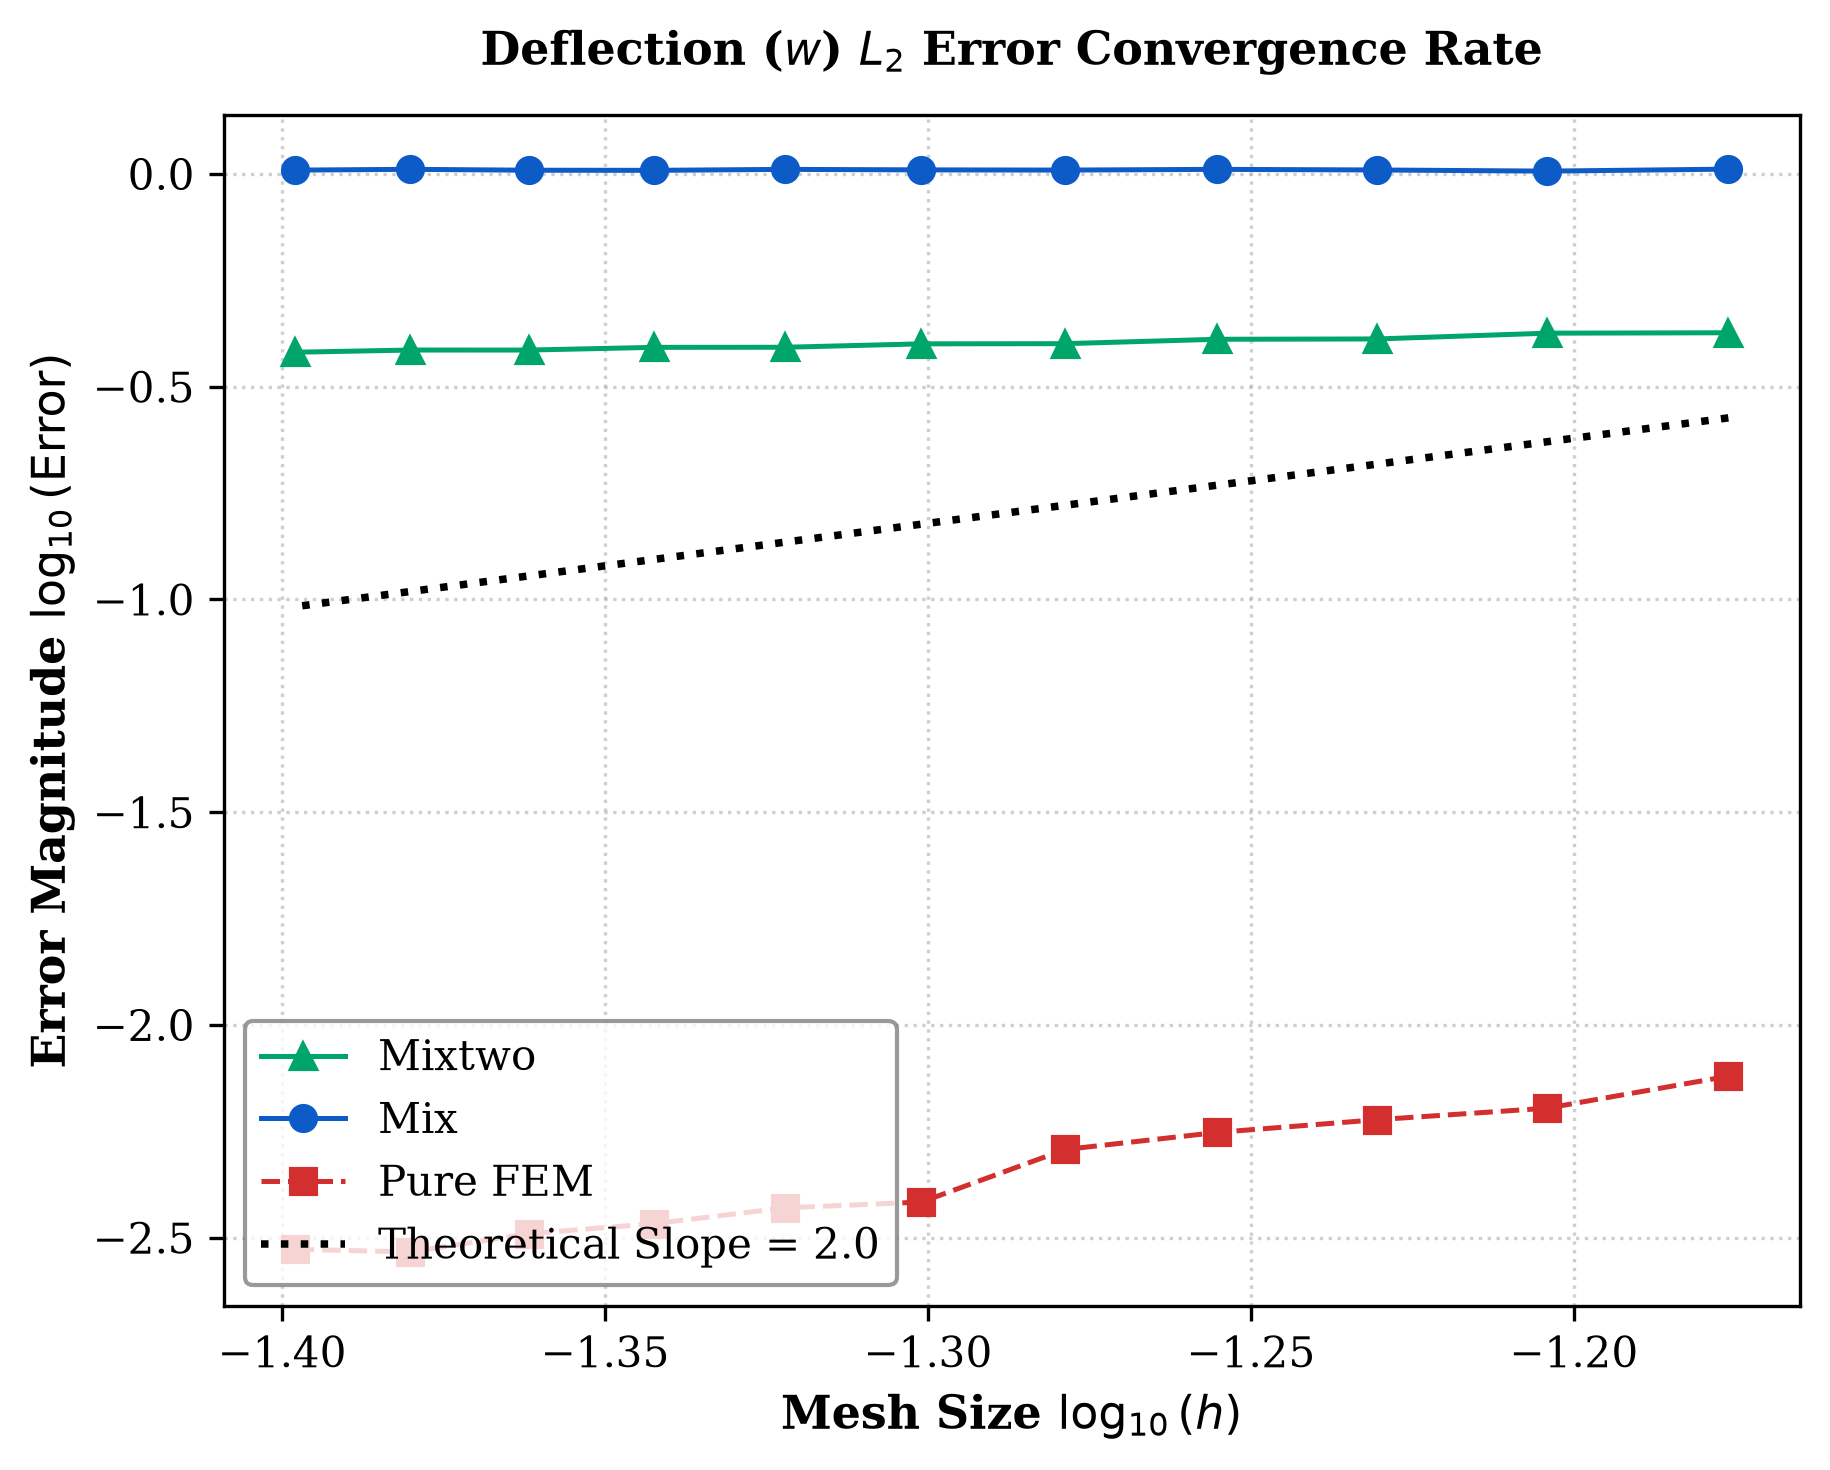
\includegraphics[width=\textwidth]{buckling_w_convergence.png}
        \caption{橫向位移場 $w$ 的相對 $L_2$ 誤差}
        \label{fig:thick_w}
    \end{subfigure}
    \hfill
    \begin{subfigure}[b]{0.48\textwidth}
        \centering
        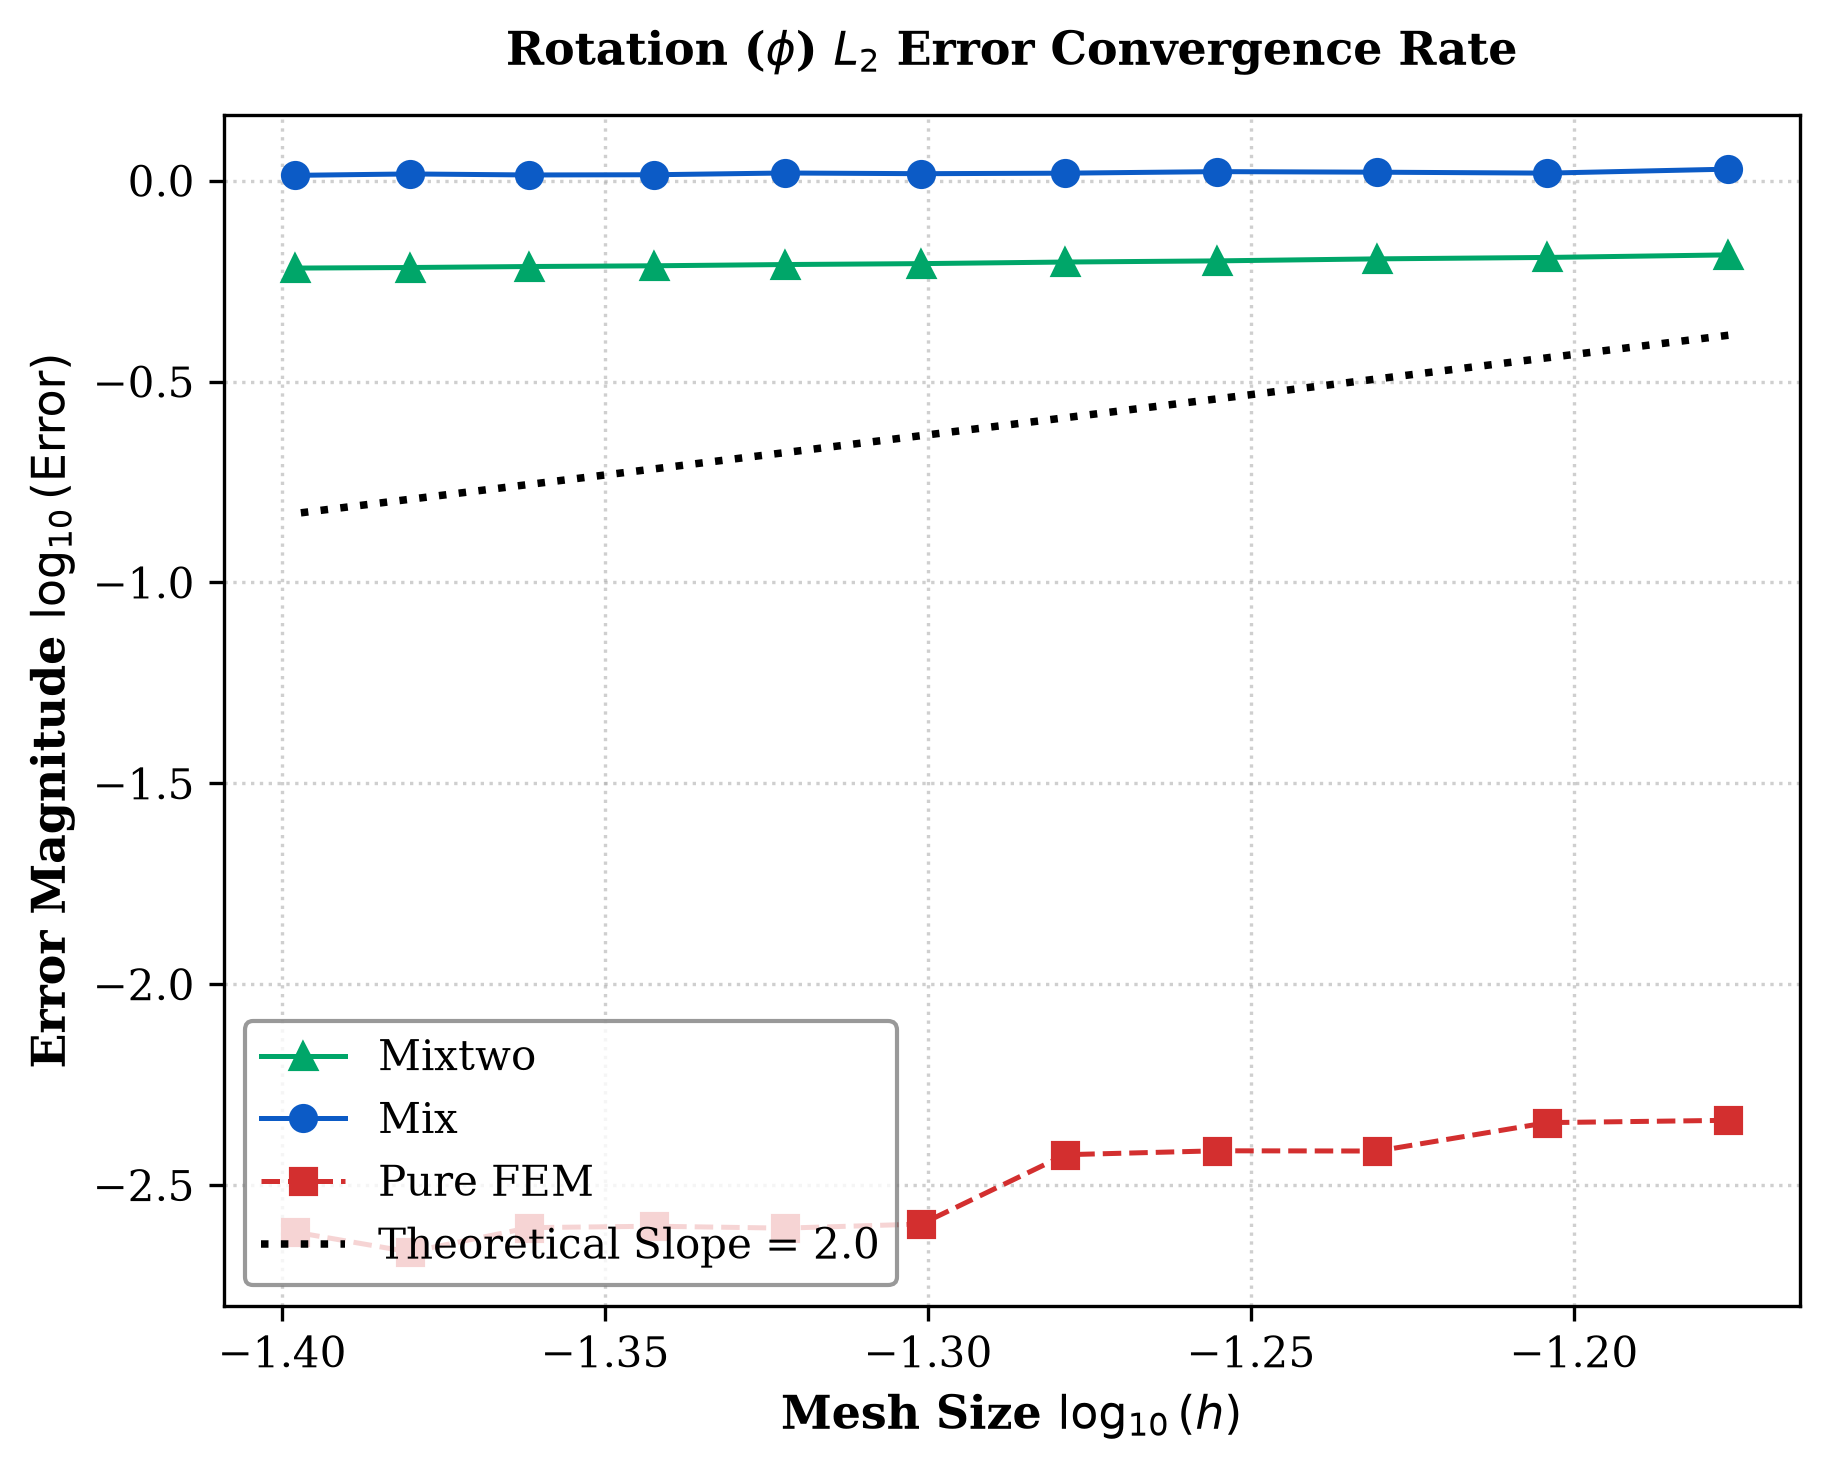
\includegraphics[width=\textwidth]{buckling_phi_convergence.png}
        \caption{截面轉角場 $\phi$ 的相對 $L_2$ 誤差}
        \label{fig:thick_phi}
    \end{subfigure}
    \caption{實驗 2 固定網格下全域高斯相對 $L_2$ 誤差隨板厚度變薄的波動曲線。}
    \label{fig:thickness_error}
\end{figure}

\subsection{數據判定與結果評判}
根據厚度效應掃描數據，對實驗 2 的計算結果進行硬核的力學評判與缺陷診斷：

\subsubsection{主要優點}
\begin{enumerate}
    \item \textbf{混合法成功消除了橫向剪切鎖死}：圖 \ref{fig:thickness_error}a 與 \ref{fig:thickness_error}b 顯示，單一網格混合法（Mix）與多網格混合法（Mixtwo）在厚度從 $0.1$ 劇烈萎縮至 $10^{-5}$ 的極薄極限過程中，全域場量 $L_2$ 誤差曲線全程保持低平與平飛，未發生發散。這證明其局部獨立插值內力場（剪力與彎矩）並透過 Schur 補碼凝聚的變分原理，成功將幾何硬約束弱化為能量弱約束，從根本上免疫了鎖死。
\end{enumerate}

\subsubsection{缺點與底層缺陷診斷}
\begin{enumerate}
    \item \textbf{傳統位移有限元（Pure FEM）完全鎖死失效}：對照數據大表可知，傳統純位移法在厚度變薄時，其解出的數值屈曲係數 $k_{\mathrm{num}}$ 迅速暴跌失真（在 $h = 10^{-5}$ 時僅剩 $0.0553$，相對誤差達 $98.61\%$）。\\
    這反映出傳統低階位移法在底層插值多項式上的本質缺陷。當厚度 $h \to 0$ 時，剪切剛度與抗彎剛度比值 $\frac{D^s}{D^b} \propto \frac{1}{h^2} \to \infty$，迫使全域必須滿足橫向剪切應變趨近於零（$\nabla w - \boldsymbol{\phi} \to \mathbf{0}$）的嚴苛約束。傳統 Q4 單元無法在內部協調該約束，導致數值剛度被無限人為放大，造成結構剛度鎖死。
    \item \textbf{混合流派全厚度區間仍受邊界剛度硬化支配}：雖然混合法消除了剪切鎖死，但在全厚度掃描中，其誤差線與特徵值絕對值仍表現出恆定的偏高，這進一步印證了第一章所述的邊界罰引數並未隨厚度自適應優化的代碼缺陷。
\end{enumerate}